% \documentclass[svgnames]{article}
% To make png: pdftopng -r 900 -alpha LucasBoston.pdf temp.png
\documentclass[svgnames,convert={density=900,size=720x600,outext=.png}]{standalone}
\usepackage{tikz}
\usetikzlibrary{calc,trees,positioning,arrows,chains,shapes.geometric,backgrounds,
  decorations.pathreplacing,decorations.pathmorphing,shapes,snakes,automata,
  matrix,shapes.symbols,mindmap,shadows,petri}
% \renewcommand{\rmdefault}{phv} % Arial
% \renewcommand{\sfdefault}{phv} % Arial
% \usepackage{amsmath} % to allow Sans font in math


\begin{document}
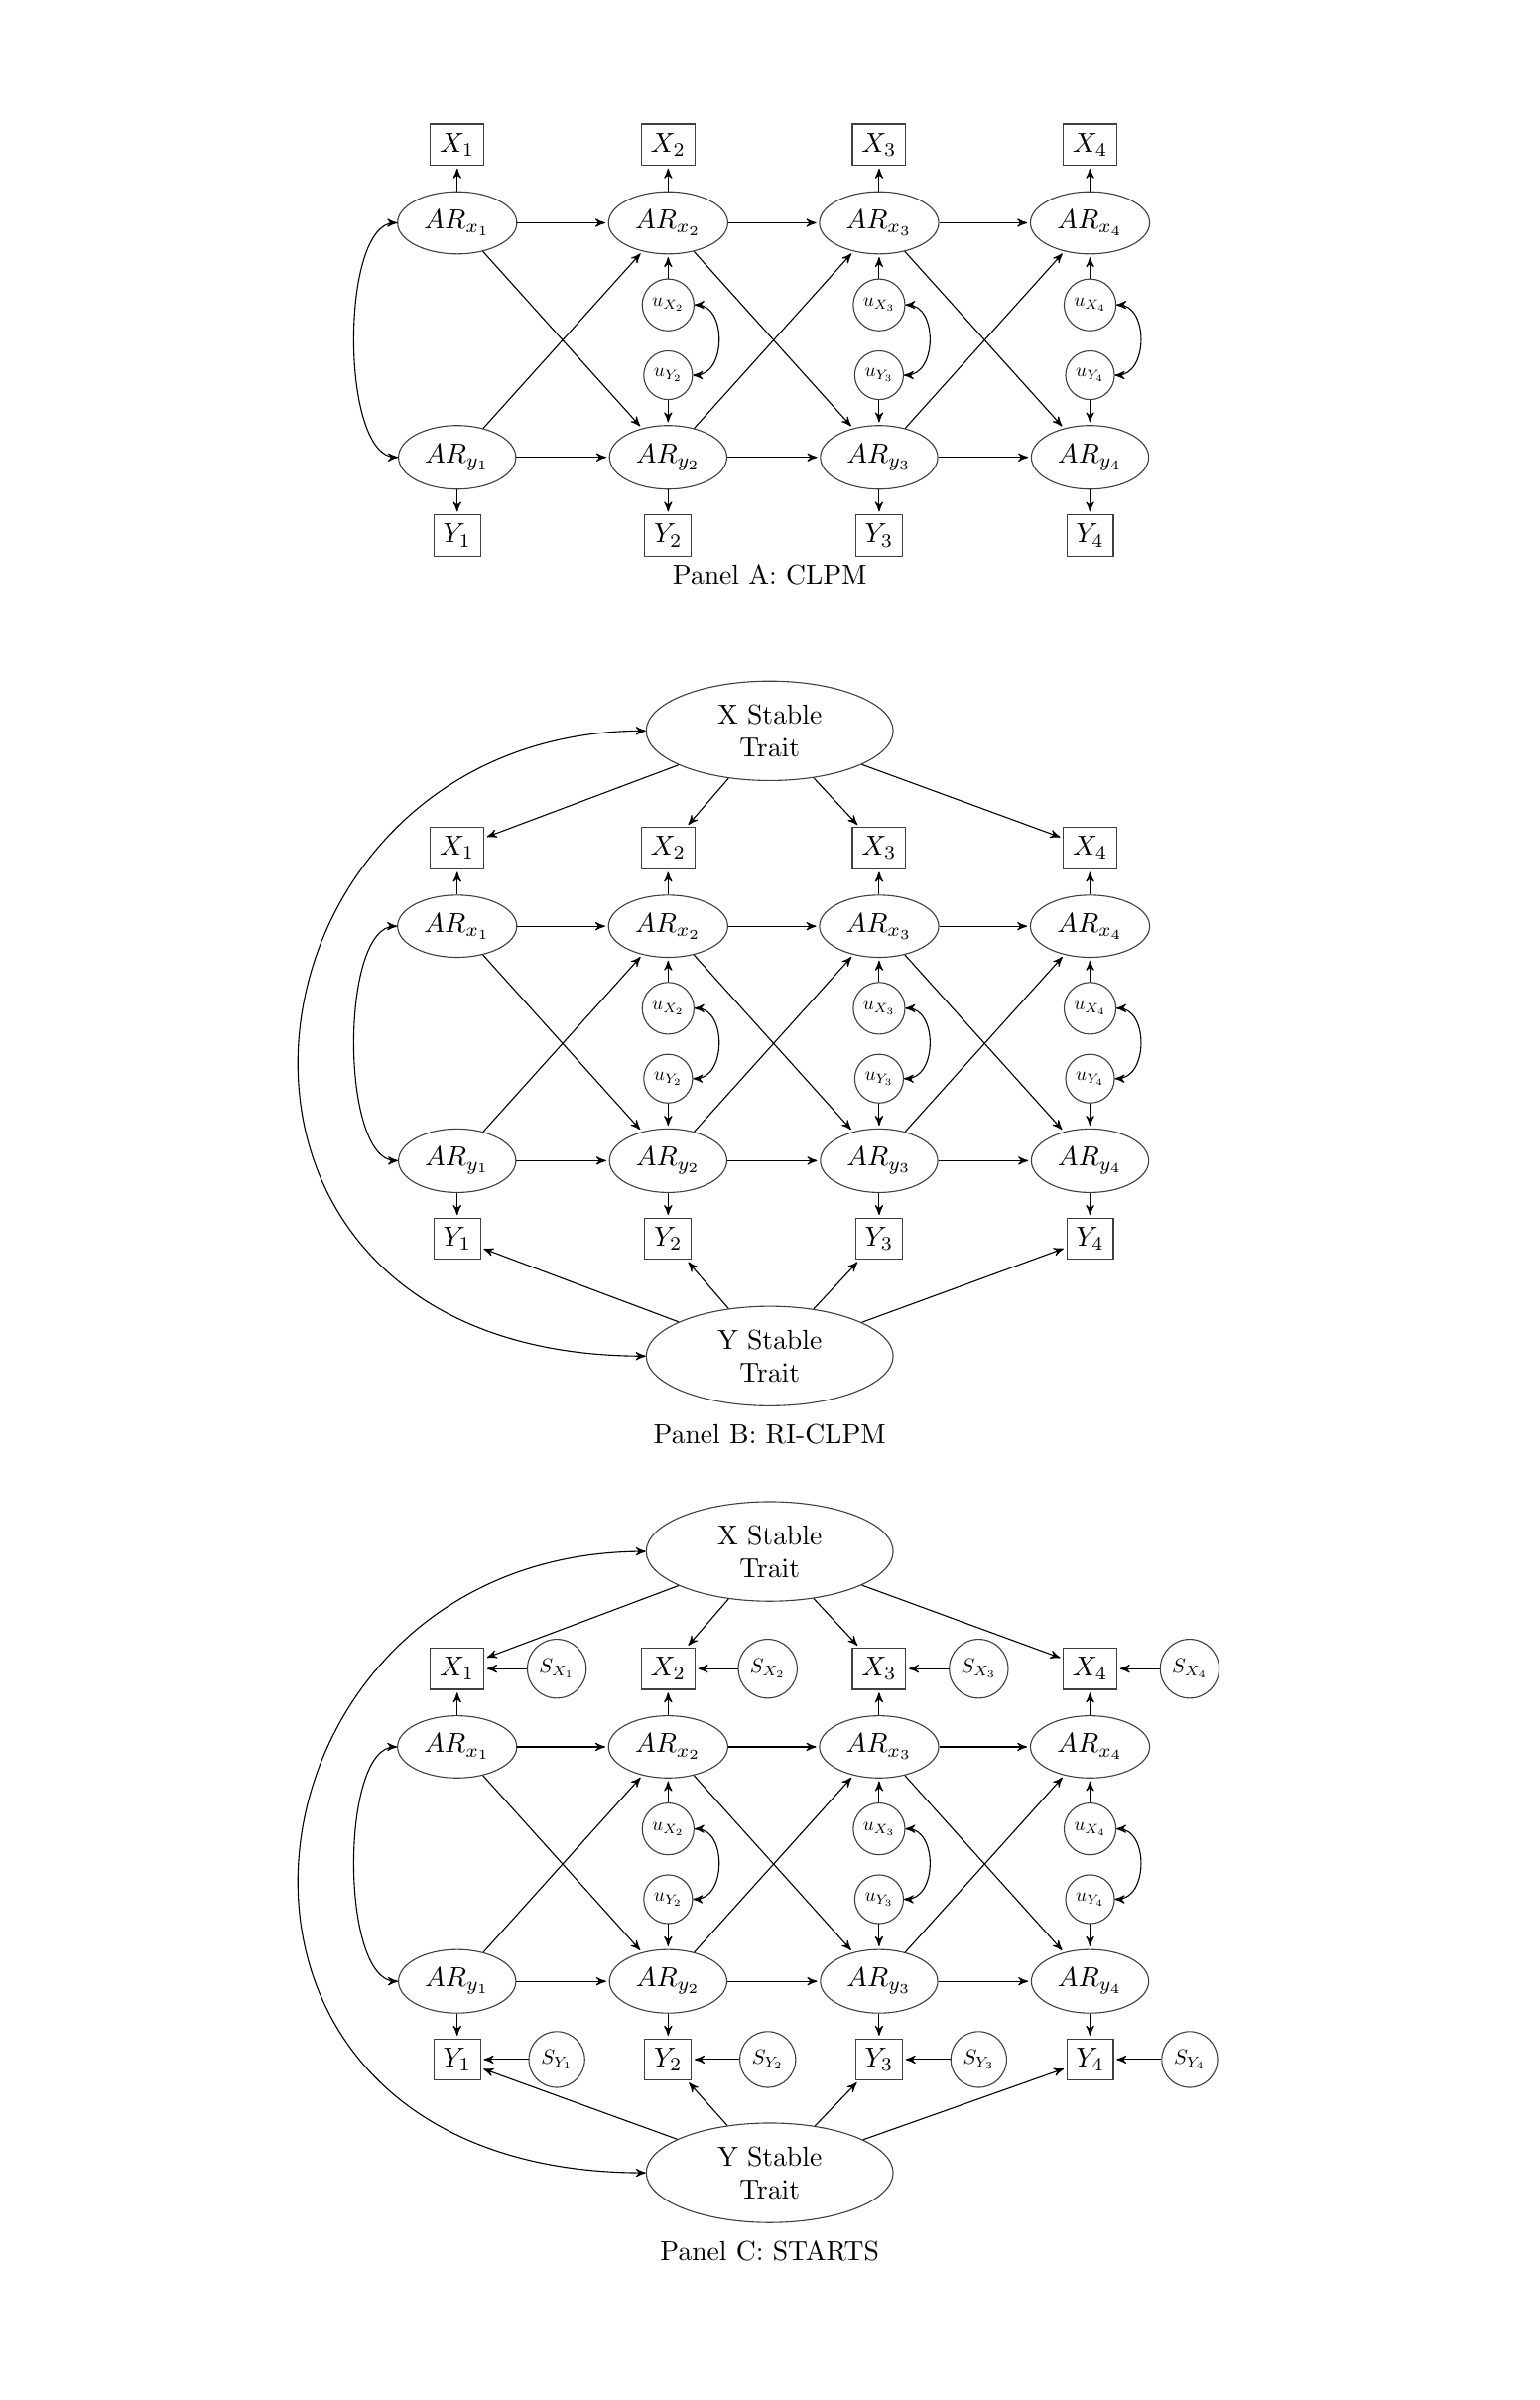
\begin{tikzpicture}[node distance=1.8cm,>=stealth',bend angle=45,auto]
  \useasboundingbox (-10,-10) rectangle (9,20);
  \tikzset{
    latentTrait/.style={ellipse,draw=black!75,minimum size=5mm, text width=20mm, align=center},
    latentAR/.style={ellipse,draw=black!75,minimum size=7mm},
    observed/.style={rectangle,draw=black!75,minimum size=5mm, align=center},
    error/.style={circle,draw=black!75,minimum size=.9mm},
    errorAR/.style={circle,draw=black!75,minimum size=.9mm, node distance=1.5cm, scale=.7},
    state/.style={circle,draw=black!75,minimum size=1mm, scale=.75, align=center, node distance=1.7cm},
    hspace/.style={node distance=2.7cm},
    vspace/.style={node distance=5cm},
    % edge styles
    indicatorDist/.style={node distance=1cm},
    errorDist/.style={node distance=.73cm},
    newARDist/.style={node distance=1.3cm},
    stabDist/.style={node distance=1cm},
    %label styles
    constraints/.style={scale=.75,above},
    constraintsb/.style={scale=.75,below},
    constraintsl/.style={scale=.75,left},
    constraintsr/.style={scale=.75,right}
  }


  % Labels
  %%% STARTS
  
  % X Vars (Health)

  \node [latentTrait] (health) at (-.5,.5)                        {X Stable Trait};
  \node [observed] (t1) at (-4.5,-1)                        {$X_1$}
  edge [pre] node[constraints] {} (health);

  \node [state] (s1) [right of=t1] {$S_{X_1}$}
  edge [post] node[constraints] {} (t1);
  
  \node [latentAR, indicatorDist] (e1) [below of=t1]                                            {$AR_{x_1}$}
  edge [post] node[constraintsl] {} (t1);
  
  \node [observed,hspace] (t2) [right of=t1]                         {$X_2$}
  edge [pre] node[constraints] {} (health) ;

  \node [state] (s2) [right of=t2] {$S_{X_2}$}
  edge [post] node[constraints] {} (t2);

  \node [latentAR, indicatorDist] (e2) [below of=t2]                                            {$AR_{x_2}$}
  edge [post] node[constraintsl] {} (t2)
  edge [pre] (e1);
  
  \node [observed, hspace] (t3) [right of=t2]                         {$X_3$}
  edge [pre] node[constraints] {} (health);

  \node [state] (s3) [right of=t3] {$S_{X_3}$}
  edge [post] node[constraints] {} (t3);

  \node [latentAR, indicatorDist] (e3) [below of=t3]                                            {$AR_{x_3}$}
  edge [post] node[constraintsl] {} (t3)
  edge [pre] (e2);
  
  \node [observed, hspace] (t4) [right of=t3]                         {$X_4$}
  edge [pre] node[constraints] {} (health);

  \node [state] (s4) [right of=t4] {$S_{X_4}$}
  edge [post] node[constraints] {} (t4);

  \node [latentAR, indicatorDist] (e4) [below of=t4]                                            {$AR_{x_4}$}
  edge [post] node[constraintsl] {} (t4)
  edge [pre] (e3);

  
  % SWB
  \node [latentTrait] (SWB) [below of=health, node distance = 7.95cm]         {Y Stable Trait};
  \node [observed, vspace] (t1s) [below of=t1] {$Y_1$}
  edge [pre] node[constraintsb] {} (SWB);
  
  \node [state] (sy1) [right of=t1s] {$S_{Y_1}$}
  edge [post] node[constraints] {} (t1s);

  \node [latentAR, indicatorDist] (e1s) [above of=t1s]                                            {$AR_{y_1}$}
  edge [post] node[constraintsl] {} (t1s)
  edge [post] (e2);
  
  \node [observed, vspace] (t2s) [below of=t2]                        {$Y_2$}
  edge [pre] node[constraintsb] {} (SWB);
  
  \node [state] (sy2) [right of=t2s] {$S_{Y_2}$}
  edge [post] node[constraints] {} (t2s);

  \node [latentAR, indicatorDist] (e2s) [above of=t2s]                                            {$AR_{y_2}$}
  edge [post] node[constraintsl] {} (t2s)
  edge [pre] (e1s)
  edge [pre] (e1)
  edge [post] (e3);
  
  \node [observed, vspace] (t3s) [below of=t3]                        {$Y_3$}
  edge [pre] node[constraintsb] {} (SWB);
  
  \node [state] (sy3) [right of=t3s] {$S_{Y_3}$}
  edge [post] node[constraints] {} (t3s);

  \node [latentAR, indicatorDist] (e3s) [above of=t3s]                                            {$AR_{y_3}$}
  edge [post] node[constraintsl] {} (t3s)
  edge [pre] (e2s)
  edge [pre] (e2)
  edge [post] (e4);
  
  \node [observed,vspace] (t4s) [below of=t4]                        {$Y_4$}
  edge [pre] node[constraintsb] {} (SWB);
  
  \node [state] (sy4) [right of=t4s] {$S_{Y_4}$}
  edge [post] node[constraints] {} (t4s);

  \node [latentAR, indicatorDist] (e4s) [above of=t4s]                                            {$AR_{y_4}$}
  edge [post] node[constraintsl] {} (t4s)
  edge [pre] (e3s)
  edge [pre] (e3);

  % Error
  \node [errorAR] (t2eh) [below of=e2] {$u_{X_2}$} edge [post] (e2);
  \node [errorAR] (t2es) [above of=e2s] {$u_{Y_2}$} edge [post] (e2s);
  \node [errorAR] (t3eh) [below of=e3] {$u_{X_3}$} edge [post] (e3);
  \node [errorAR] (t3es) [above of=e3s] {$u_{Y_3}$} edge [post] (e3s);
  \node [errorAR] (t4eh) [below of=e4] {$u_{X_4}$} edge [post] (e4);
  \node [errorAR] (t4es) [above of=e4s] {$u_{Y_4}$} edge [post] (e4s);


  % Correlations
  \draw [<->] (SWB) .. controls +(left:8cm) and +
  (left:7cm) .. node[sloped,above] {} (health);
  \draw [<->] (e1s) .. controls + (left:1.5cm) and +
  (left:1.5cm) .. (e1);
  \draw [<->] (t2es) .. controls + (right:.75cm) and +
  (right:.75cm) ..  (t2eh);
  \draw [<->] (t3es) .. controls + (right:.75cm) and +
  (right:.75cm) ..  (t3eh);
  \draw [<->] (t4es) .. controls + (right:.75cm) and +
  (right:.75cm) .. node[above,rotate=-90,scale=.75] {}  (t4eh);

  % Panel Label
  \node (label1) [below of=SWB, node distance=1cm] {Panel C: STARTS};


  % Stabilities


  %%% RI-CLPM

    % X Vars (Health)

  \node [latentTrait] (rihealth) at (-.5,11)                        {X Stable Trait};
  \node [observed] (rit1) at (-4.5,9.5)                        {$X_1$}
  edge [pre] node[constraints] {} (rihealth);

  % \node [state] (ris1) [right of=rit1] {$S_{X_1}$}
  % edge [post] node[constraints] {1} (rit1);
  
  \node [latentAR, indicatorDist] (rie1) [below of=rit1]                                            {$AR_{x_1}$}
  edge [post] node[constraintsl] {} (rit1);
  
  \node [observed,hspace] (rit2) [right of=rit1]                         {$X_2$}
  edge [pre] node[constraints] {} (rihealth) ;

  % \node [state] (ris2) [right of=rit2] {$S_{X_2}$}
  % edge [post] node[constraints] {1} (rit2);

  \node [latentAR, indicatorDist] (rie2) [below of=rit2]                                            {$AR_{x_2}$}
  edge [post] node[constraintsl] {} (rit2)
  edge [pre] (rie1);
  
  \node [observed, hspace] (rit3) [right of=rit2]                         {$X_3$}
  edge [pre] node[constraints] {} (rihealth);

  % \node [state] (ris3) [right of=rit3] {$S_{X_3}$}
  % edge [post] node[constraints] {1} (rit3);

  \node [latentAR, indicatorDist] (rie3) [below of=rit3]                                            {$AR_{x_3}$}
  edge [post] node[constraintsl] {} (rit3)
  edge [pre] (rie2);
  
  \node [observed, hspace] (rit4) [right of=rit3]                         {$X_4$}
  edge [pre] node[constraints] {} (rihealth);

  % \node [state] (ris4) [right of=rit4] {$S_{X_4}$}
  % edge [post] node[constraints] {1} (rit4);

  \node [latentAR, indicatorDist] (rie4) [below of=rit4]                                            {$AR_{x_4}$}
  edge [post] node[constraintsl] {} (rit4)
  edge [pre] (rie3);

  
  % SWB
  \node [latentTrait] (riSWB) [below of=rihealth, node distance = 8cm]         {Y Stable Trait};
  \node [observed, vspace] (rit1s) [below of=rit1] {$Y_1$}
  edge [pre] node[constraintsb] {} (riSWB);
  
  % \node [state] (risy1) [right of=rit1s] {$S_{Y_1}$}
  % edge [post] node[constraints] {1} (rit1s);

  \node [latentAR, indicatorDist] (rie1s) [above of=rit1s]                                            {$AR_{y_1}$}
  edge [post] node[constraintsl] {} (rit1s)
  edge [post] (rie2);
  
  \node [observed, vspace] (rit2s) [below of=rit2]                        {$Y_2$}
  edge [pre] node[constraintsb] {} (riSWB);
  
  % \node [state] (risy2) [right of=rit2s] {$S_{Y_2}$}
  % edge [post] node[constraints] {1} (rit2s);

  \node [latentAR, indicatorDist] (rie2s) [above of=rit2s]                                            {$AR_{y_2}$}
  edge [post] node[constraintsl] {} (rit2s)
  edge [pre] (rie1s)
  edge [pre] (rie1)
  edge [post] (rie3);
  
  \node [observed, vspace] (rit3s) [below of=rit3]                        {$Y_3$}
  edge [pre] node[constraintsb] {} (riSWB);
  
  % \node [state] (risy3) [right of=rit3s] {$S_{Y_3}$}
  % edge [post] node[constraints] {1} (rit3s);

  \node [latentAR, indicatorDist] (rie3s) [above of=rit3s]                                            {$AR_{y_3}$}
  edge [post] node[constraintsl] {} (rit3s)
  edge [pre] (rie2s)
  edge [pre] (rie2)
  edge [post] (rie4);
  
  \node [observed,vspace] (rit4s) [below of=rit4]                        {$Y_4$}
  edge [pre] node[constraintsb] {} (riSWB);
  
  % \node [state] (risy4) [right of=rit4s] {$S_{Y_4}$}
  % edge [post] node[constraints] {1} (rit4s);

  \node [latentAR, indicatorDist] (rie4s) [above of=rit4s]                                            {$AR_{y_4}$}
  edge [post] node[constraintsl] {} (rit4s)
  edge [pre] (rie3s)
  edge [pre] (rie3);

  % Error
  \node [errorAR] (rit2eh) [below of=rie2] {$u_{X_2}$} edge [post] (rie2);
  \node [errorAR] (rit2es) [above of=rie2s] {$u_{Y_2}$} edge [post] (rie2s);
  \node [errorAR] (rit3eh) [below of=rie3] {$u_{X_3}$} edge [post] (rie3);
  \node [errorAR] (rit3es) [above of=rie3s] {$u_{Y_3}$} edge [post] (rie3s);
  \node [errorAR] (rit4eh) [below of=rie4] {$u_{X_4}$} edge [post] (rie4);
  \node [errorAR] (rit4es) [above of=rie4s] {$u_{Y_4}$} edge [post] (rie4s);


  % Correlations
  \draw [<->] (riSWB) .. controls +(left:8cm) and +
  (left:7cm) .. node[sloped,above] {} (rihealth);
  \draw [<->] (rie1s) .. controls + (left:1.5cm) and +
  (left:1.5cm) .. (rie1);
  \draw [<->] (rit2es) .. controls + (right:.75cm) and +
  (right:.75cm) ..  (rit2eh);
  \draw [<->] (rit3es) .. controls + (right:.75cm) and +
  (right:.75cm) ..  (rit3eh);
  \draw [<->] (rit4es) .. controls + (right:.75cm) and +
  (right:.75cm) .. node[above,rotate=-90,scale=.75] {}  (rit4eh);

  % Panel Label
  \node (label2) [below of=riSWB, node distance=1cm] {Panel B: RI-CLPM};


  %%% CLPM

      % X Vars (Health)

  \node [observed] (clt1) at (-4.5,18.5)                        {$X_1$};	

  \node [latentAR, indicatorDist] (cle1) [below of=clt1]                                            {$AR_{x_1}$}
  edge [post] node[constraintsl] {} (clt1);
  
  \node [observed,hspace] (clt2) [right of=clt1]                         {$X_2$};

  \node [latentAR, indicatorDist] (cle2) [below of=clt2]                                            {$AR_{x_2}$}
  edge [post] node[constraintsl] {} (clt2)
  edge [pre] (cle1);
  
  \node [observed, hspace] (clt3) [right of=clt2]                         {$X_3$};
  
  \node [latentAR, indicatorDist] (cle3) [below of=clt3]                                            {$AR_{x_3}$}
  edge [post] node[constraintsl] {} (clt3)
  edge [pre] (cle2);
  
  \node [observed, hspace] (clt4) [right of=clt3]                         {$X_4$};

  \node [latentAR, indicatorDist] (cle4) [below of=clt4]                                            {$AR_{x_4}$}
  edge [post] node[constraintsl] {} (clt4)
  edge [pre] (cle3);

  
  % SWB
  \node [observed, vspace] (clt1s) [below of=clt1] {$Y_1$};

  \node [latentAR, indicatorDist] (cle1s) [above of=clt1s]                                            {$AR_{y_1}$}
  edge [post] node[constraintsl] {} (clt1s)
  edge [post] (cle2);
  
  \node [observed, vspace] (clt2s) [below of=clt2]                        {$Y_2$};

  \node [latentAR, indicatorDist] (cle2s) [above of=clt2s]                                            {$AR_{y_2}$}
  edge [post] node[constraintsl] {} (clt2s)
  edge [pre] (cle1s)
  edge [pre] (cle1)
  edge [post] (cle3);
  
  \node [observed, vspace] (clt3s) [below of=clt3]                        {$Y_3$};

  \node [latentAR, indicatorDist] (cle3s) [above of=clt3s]                                            {$AR_{y_3}$}
  edge [post] node[constraintsl] {} (clt3s)
  edge [pre] (cle2s)
  edge [pre] (cle2)
  edge [post] (cle4);
  
  \node [observed,vspace] (clt4s) [below of=clt4]                        {$Y_4$};

  \node [latentAR, indicatorDist] (cle4s) [above of=clt4s]                                            {$AR_{y_4}$}
  edge [post] node[constraintsl] {} (clt4s)
  edge [pre] (cle3s)
  edge [pre] (cle3);

  % Error
  \node [errorAR] (clt2eh) [below of=cle2] {$u_{X_2}$} edge [post] (cle2);
  \node [errorAR] (clt2es) [above of=cle2s] {$u_{Y_2}$} edge [post] (cle2s);
  \node [errorAR] (clt3eh) [below of=cle3] {$u_{X_3}$} edge [post] (cle3);
  \node [errorAR] (clt3es) [above of=cle3s] {$u_{Y_3}$} edge [post] (cle3s);
  \node [errorAR] (clt4eh) [below of=cle4] {$u_{X_4}$} edge [post] (cle4);
  \node [errorAR] (clt4es) [above of=cle4s] {$u_{Y_4}$} edge [post] (cle4s);


  % Correlations
  \draw [<->] (cle1s) .. controls + (left:1.5cm) and +
  (left:1.5cm) .. (cle1);
  \draw [<->] (clt2es) .. controls + (right:.75cm) and +
  (right:.75cm) ..  (clt2eh);
  \draw [<->] (clt3es) .. controls + (right:.75cm) and +
  (right:.75cm) ..  (clt3eh);
  \draw [<->] (clt4es) .. controls + (right:.75cm) and +
  (right:.75cm) .. node[above,rotate=-90,scale=.75] {}  (clt4eh);

  % Panel Label
  \node (label3) [above of=label2, node distance=11cm] {Panel A: CLPM};
  


  
\end{tikzpicture}
\end{document}